\chapter{Implementación}

En este capítulo se detalla la implementación de la plataforma desarrollada, describiendo las decisiones técnicas, herramientas y metodologías empleadas para materializar los objetivos planteados. La arquitectura del sistema se fundamenta en la separación clara entre el backend, responsable del procesamiento de datos y la lógica principal de la aplicación, y el frontend, encargado de la presentación e interacción con el usuario. Esta aproximación modular facilita el mantenimiento, escalabilidad y futuras extensiones del sistema.

\begin{figure}[H]
  \centering
  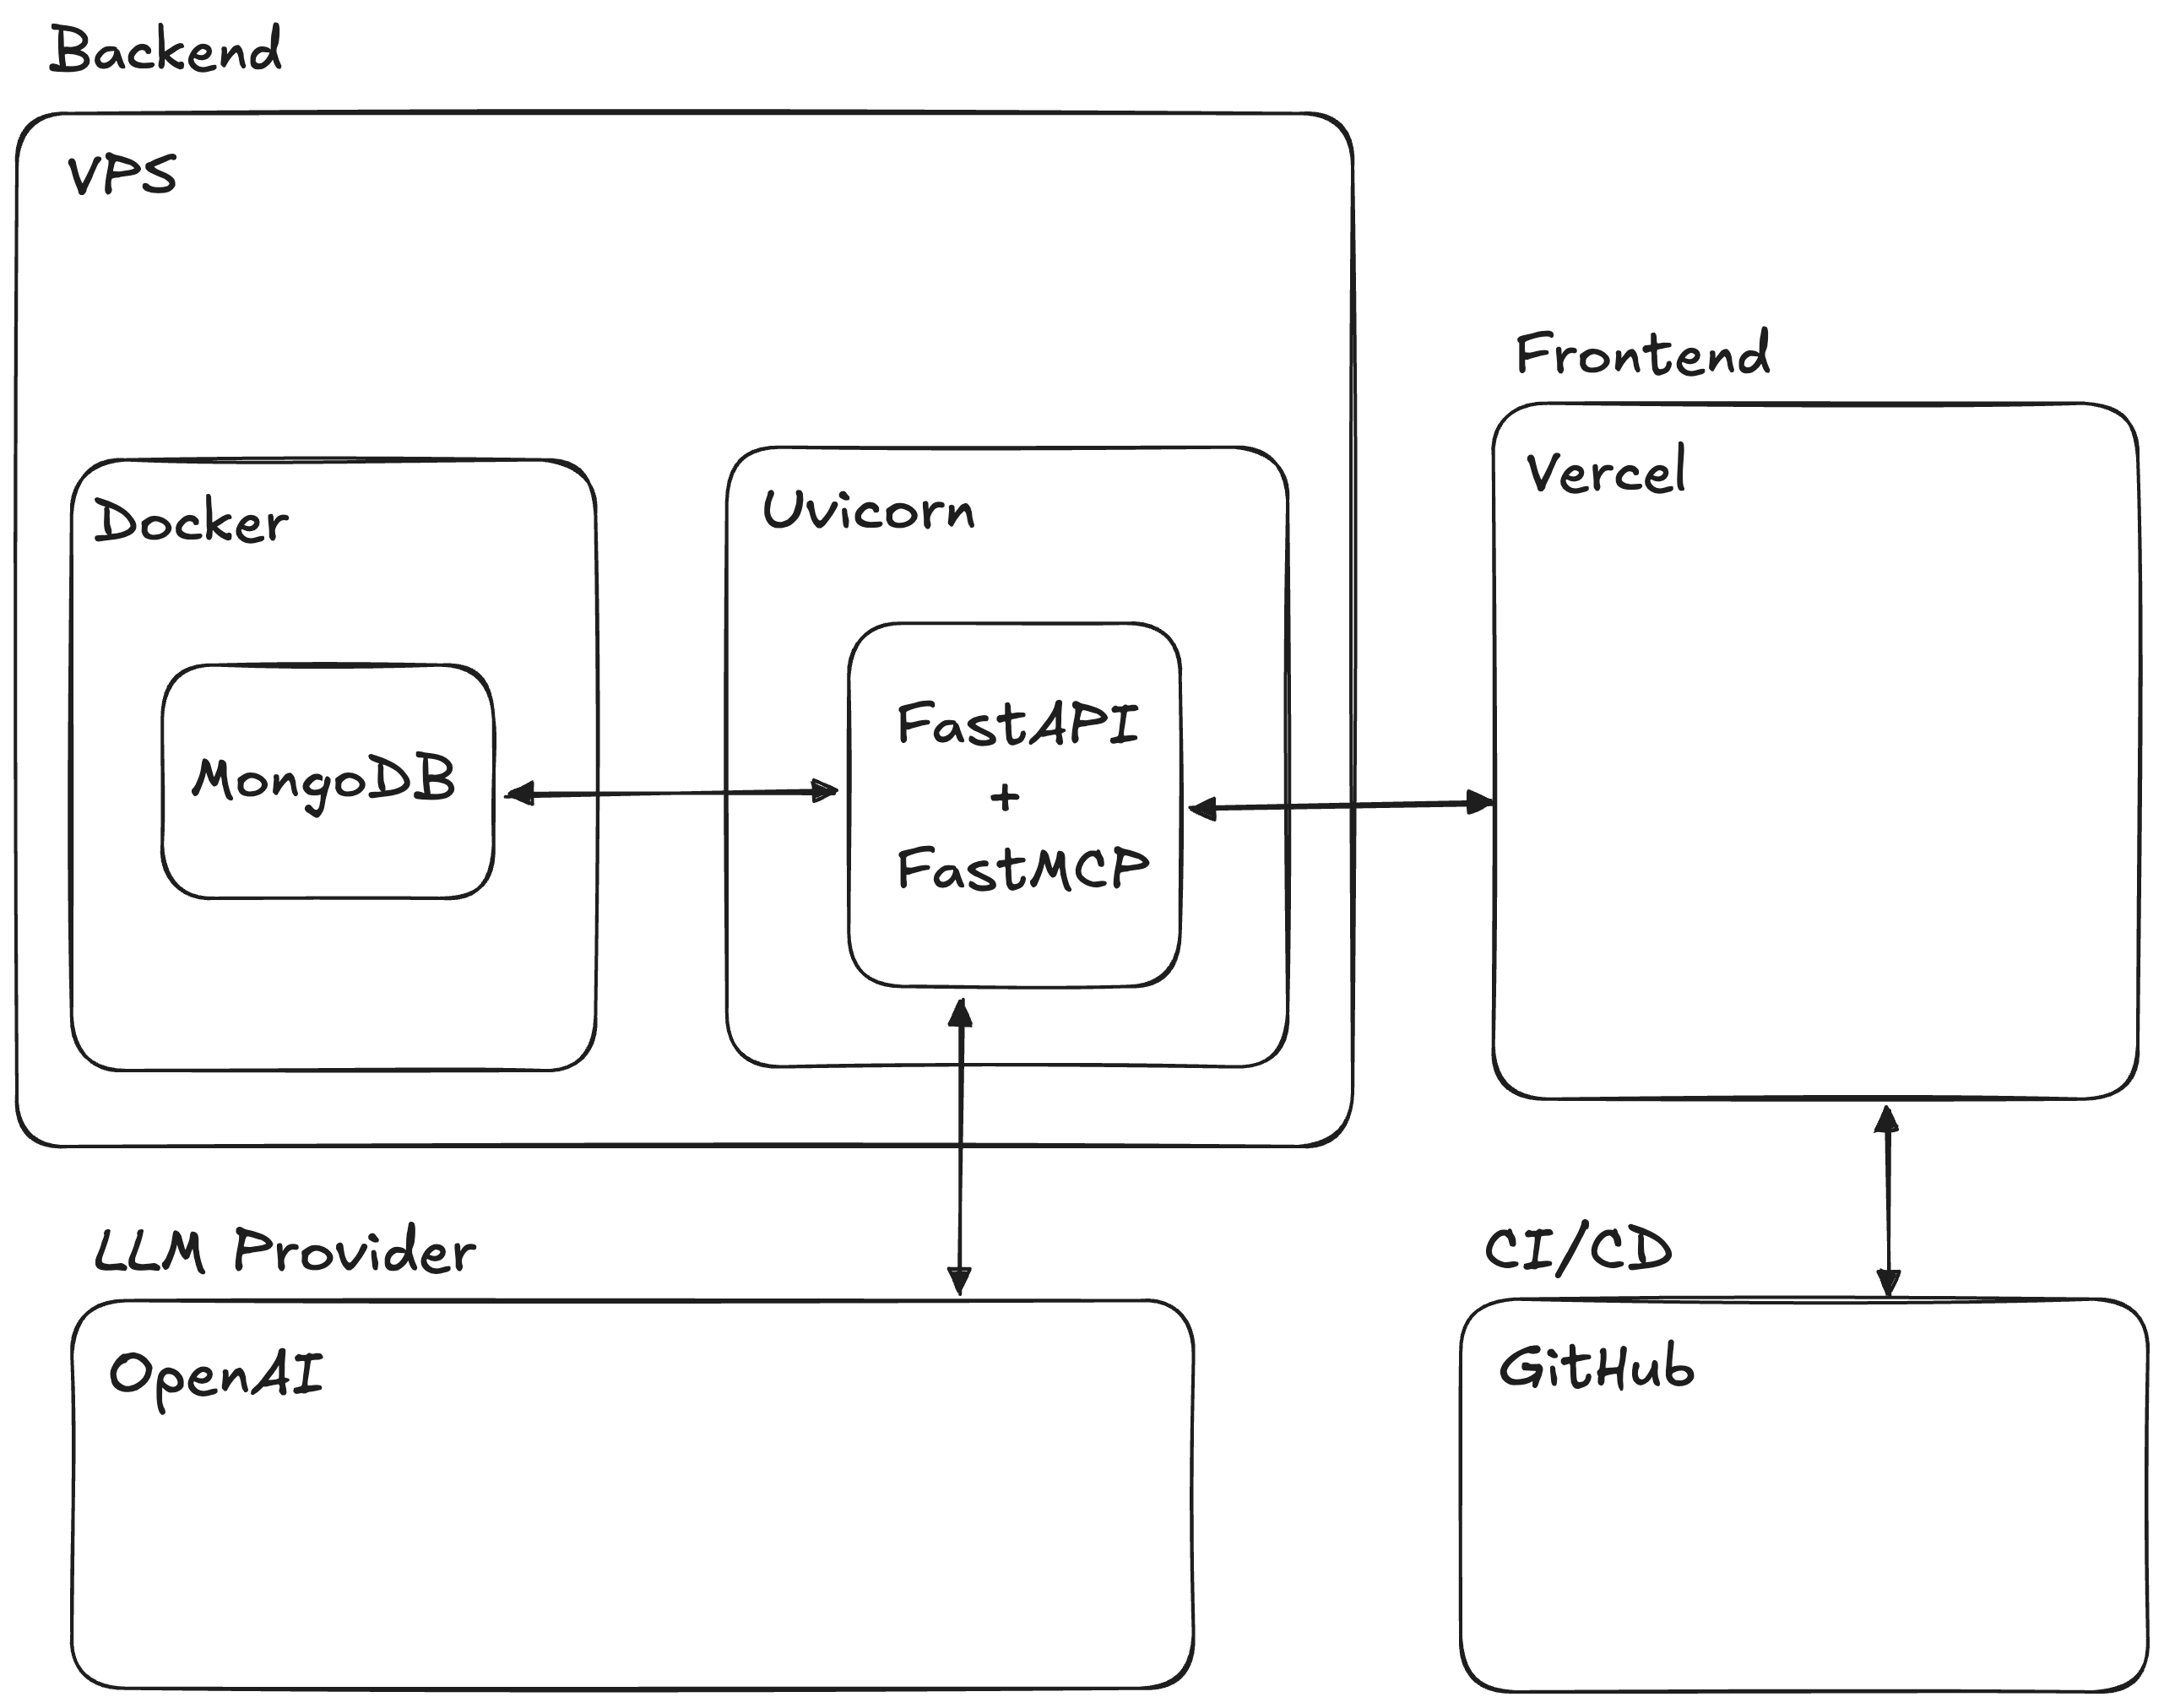
\includegraphics[width=0.9\textwidth]{imagenes/arch1.png}
  \caption{Arquitectura de la aplicación}
  \label{fig:arch1}
\end{figure}

\section{Backend}

El backend constituye el núcleo de la lógica de este trabajo. Se puede dividir en dos elementos: la base de datos MIMIC-IV almacenada en MongoDB con Docker, y la API RESTful con FastAPI que consulta datos, los procesa y los devuelve al cliente. Todo se aloja en un servidor personal y se accede por HTTPS gracias a Cloudflare Tunnels.

%\subsection{Almacenamiento de MIMIC-IV en MongoDB}
\subsection{MIMIC-IV en MongoDB}


Una de las tareas técnicas fundamentales del proyecto ha sido la migración del conjunto de datos desde su formato original en CSV a una base de datos MongoDB. MIMIC-IV se distribuye como un conjunto de archivos CSV comprimidos organizados en dos módulos principales: \texttt{hosp} (datos hospitalarios) e \texttt{icu} (datos de cuidados intensivos), junto con diccionarios de códigos y metadatos complementarios.


El proceso de migración se implementó mediante scripts de Python utilizando la librería \texttt{pandas} para la lectura de archivos CSV y \texttt{pymongo} para la inserción en MongoDB. Cada fila del CSV se convierte en un archivo JSON en MongoDB, cada columna es un campo del documento, y cada archivo CSV completo acaba siendo una colección de documentos. El procesamiento se hizo por chuncks para evitar el desbordamiento de memoria, que fue un problema recurrente debido a la cantidad masiva de datos.


Tras la importación, resultaron las siguientes colecciones:




Para el despliegue de MongoDB se utilizan dos contenedores Docker, en distintos puertos, uno para la versión demo del conjunto de datos, y otro para la versión completa, facilitando la realización de pruebas. Como apoyo al desarrollo, y también en forma de contenedores, se despliegan las herramientas de interfaz gráfica: Portainer para Docker\cite{portainer_ce} y Mongo Express para las bases de datos\cite{mongo_express}. 

\begin{figure}[H]
  \centering
  \fbox{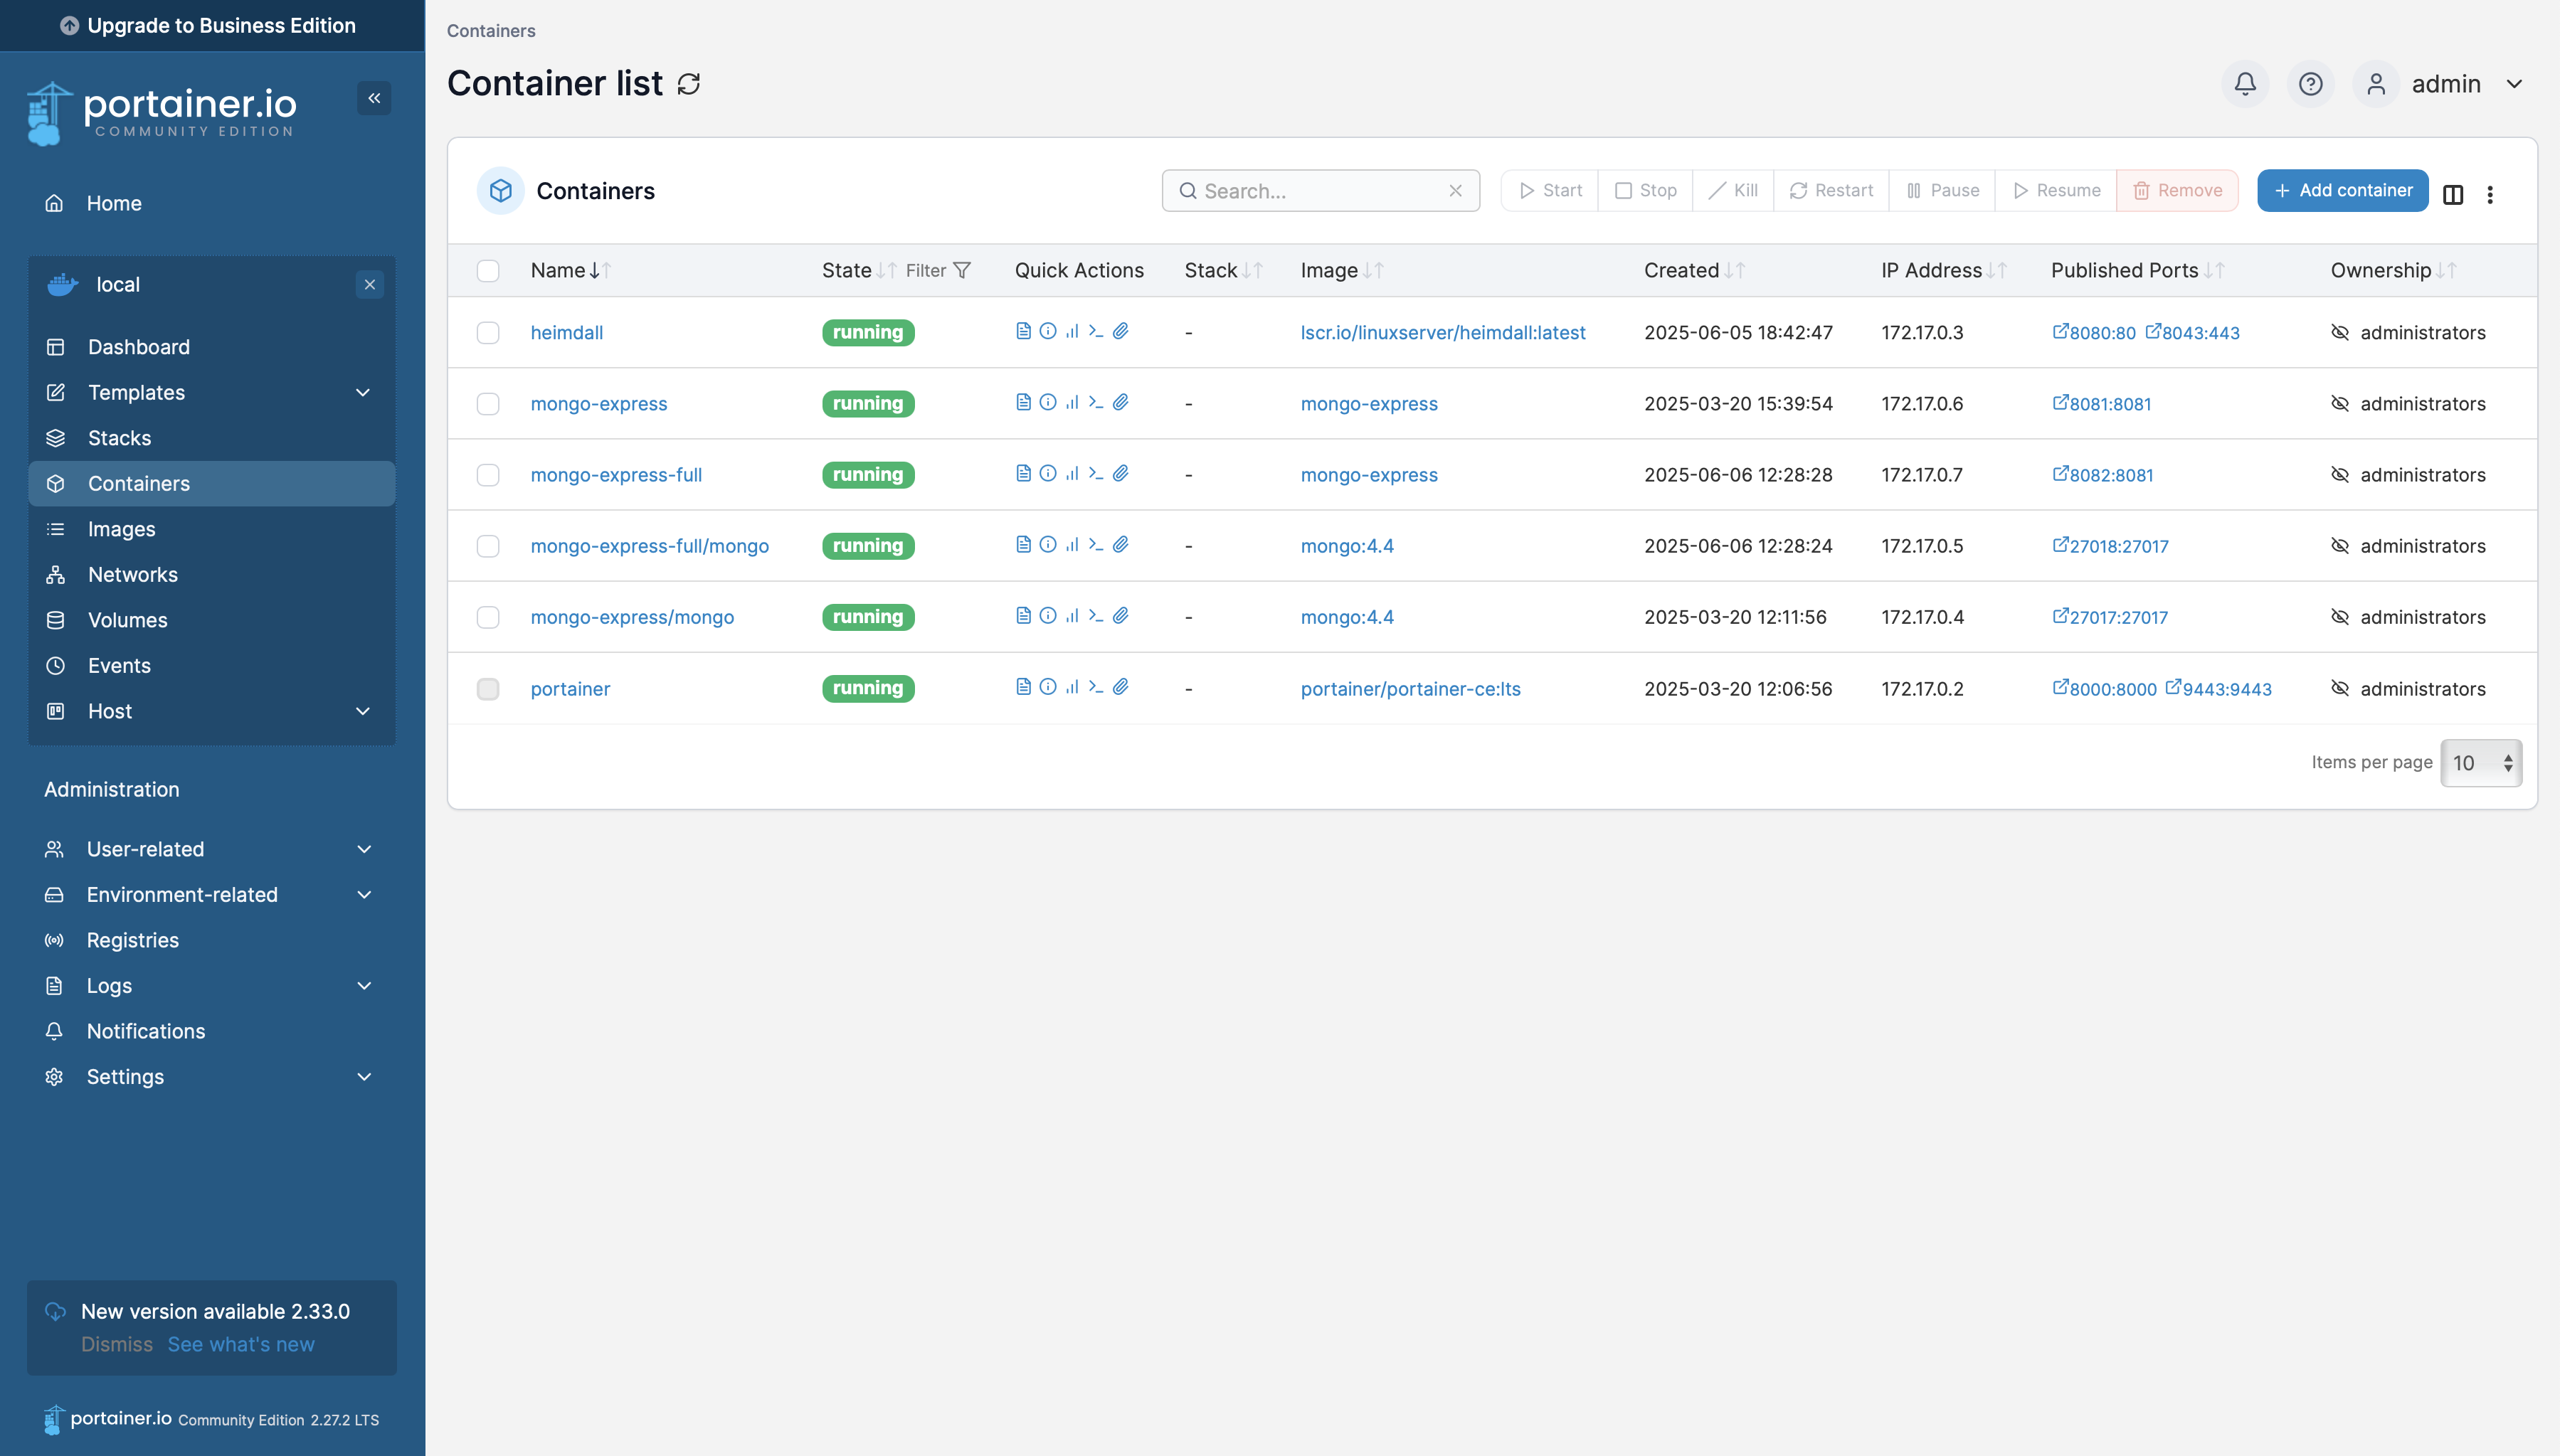
\includegraphics[width=1\textwidth]{imagenes/screenshot1.png}}
  \caption{Captura de pantalla de Portainer}
  \label{fig:screenshot1s}
\end{figure}


\begin{figure}[H]
  \centering
  \fbox{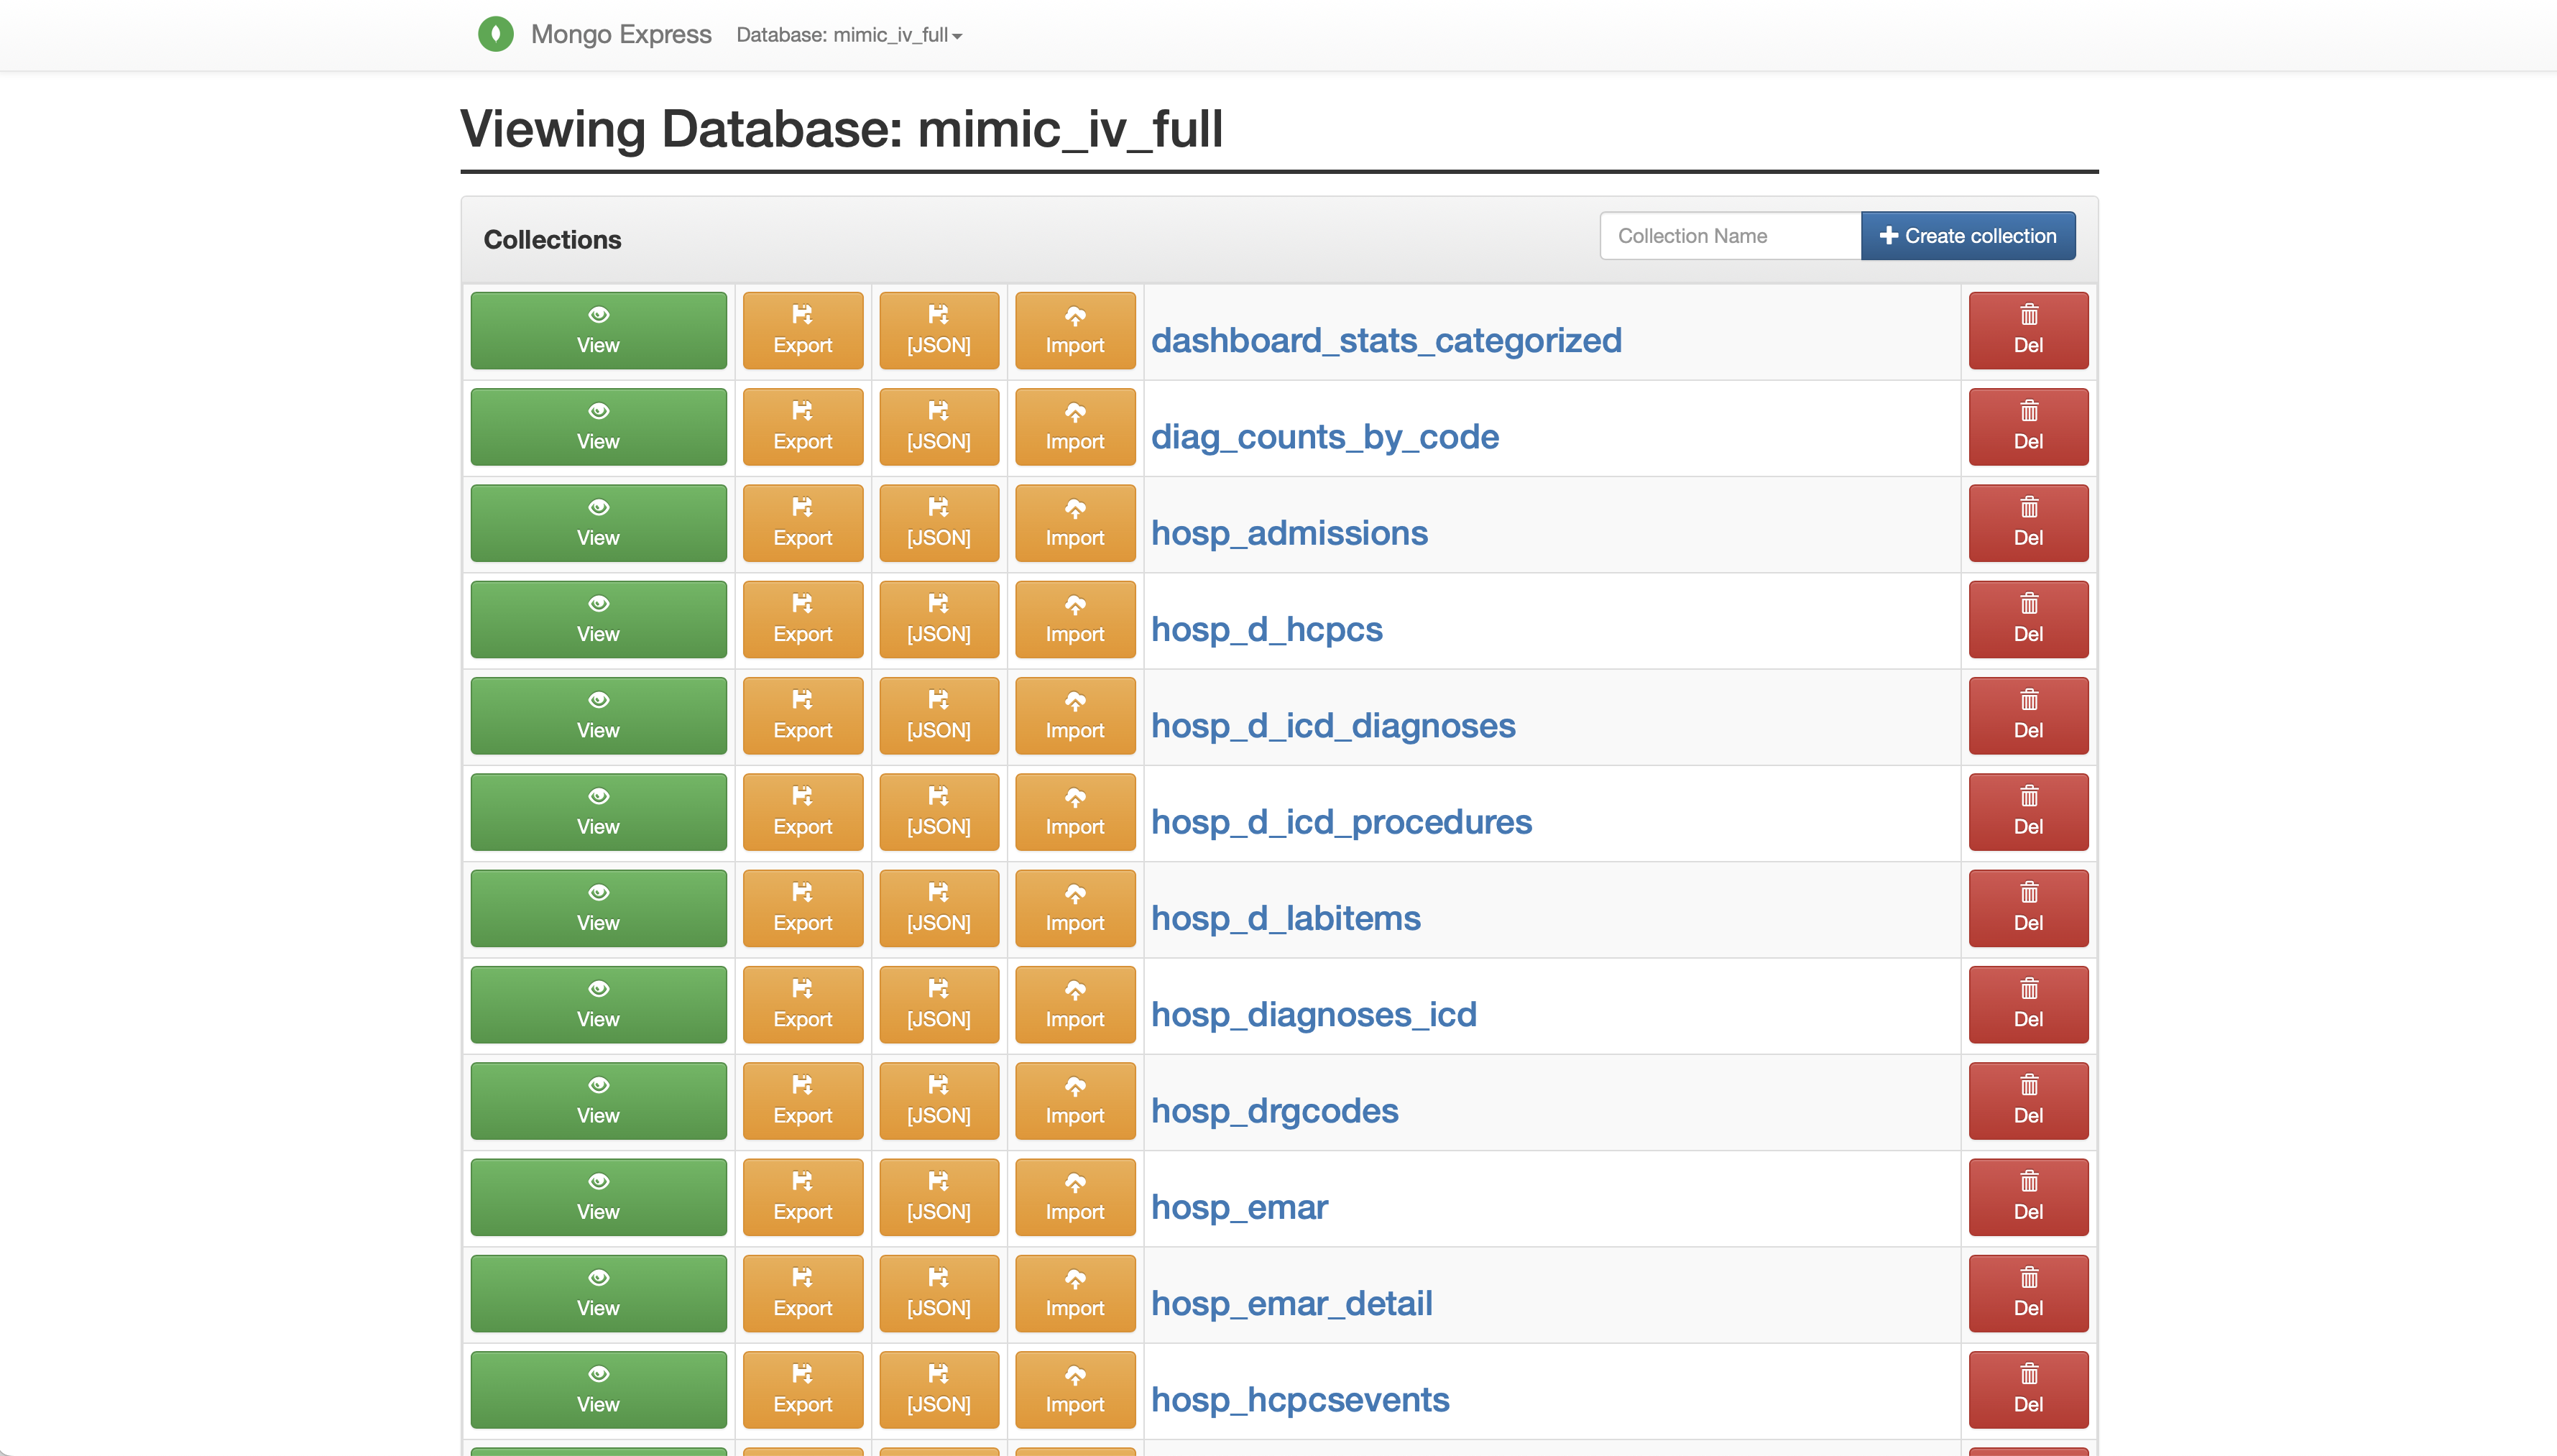
\includegraphics[width=1\textwidth]{imagenes/screenshot2.png}}
  \caption{Captura de pantalla de Mongo Express}
  \label{fig:screenshot2}
\end{figure}


\subsection{API RESTful}

La API que obtiene, procesa y sirve los datos está construida sobre FastAPI, un framework moderno que combina alto rendimiento con una sintaxis intuitiva y generación automática de documentación. Para separar responsabilidades, el código se estructura de la siguiente forma:

\begin{itemize}
\item \textbf{Capa de datos:} El módulo \texttt{db/mongo.py} encapsula la conexión a MongoDB y proporciona funciones de utilidad.
\item \textbf{Capa de rutas:} Organizadas por funcionalidad en el directorio \texttt{routes/}, incluyen endpoints para pacientes, dashboard, gráficos y chat.
\item \textbf{Capa de aplicación:} El archivo principal \texttt{main.py} configura la aplicación, middleware CORS y el enrutamiento.
\end{itemize}

Utilizamos Uvicorn como servidor ASGI (Asynchronous Server Gateway Interface) que escuchará las peticiones a los endpoints. 

(...completar con las demas cosas que se usen para la IA)

(...poner imagen esquemita de los archivos orden y tal?)


\subsection{Inteligencia Artificial}

Para este proyecto hemos elegido trabajar con los modelos de texto de OpenAI, mediante su libreria para Python.


\section{Frontend}

El frontend está desarrollado utilizando Next.js 15 y TypeScript. Se aloja la web en Vercel por su extrema facilidad de uso, plan gratuito, auto-deploy desde GitHub, gran optimización y CDN global. La arquitectura se basa en componentes reutilizables y páginas especializadas que consumen la API del backend.

@todo: hablar de la clasificación de los datos en categorías: demográficos y admisiones, cuidados intensivos, laboratorio y medicamentos, diagnósticos y procedimientos, y flujos hospitalarios.

\subsection{Arquitectura de Componentes}

La estructura del frontend sigue las convenciones de Next.js con el nuevo App Router, organizando el código en:

\begin{itemize}
\item \textbf{Páginas:} Ubicadas en \texttt{src/app/}, incluyen la página principal, dashboard, búsqueda de pacientes, chat y visualizaciones específicas.
\item \textbf{Componentes:} En \texttt{src/components/}, contienen elementos reutilizables como el header, componentes de gráficos y elementos de UI.
\item \textbf{Hooks personalizados:} En \texttt{src/hooks/}, encapsulan lógica específica como el monitoreo de salud del backend.
\item \textbf{Tipos TypeScript:} En \texttt{src/types/}, definen las interfaces de datos para garantizar type safety.
\end{itemize}

Se utiliza Lucide React para iconografía consistente y Tailwind CSS para el diseño.

\subsection{Visualización de Datos}

Se ha implementado una estrategia progresiva utilizando múltiples librerías según la complejidad requerida:

\begin{itemize}
\item \textbf{Observable Plot:} Para gráficos estándar como distribuciones de edad y estadísticas básicas, aprovechando su API declarativa y soluciones preestablecidas.
\item \textbf{D3.js:} Para visualizaciones complejas que requieren control granular sobre el renderizado y la interactividad.
\end{itemize}

(...esto habra que revisarlo y cambiarlo cuando esten hechos ya todos los graficos acabados....)

Los componentes de visualización están diseñados como elementos autónomos que consumen datos de la API y manejan sus propios estados de carga y error. Esta aproximación facilita la reutilización y el testing individual de cada visualización.

Estos son los gráficos que se han implementado:



\begin{figure}[H]
  \centering
  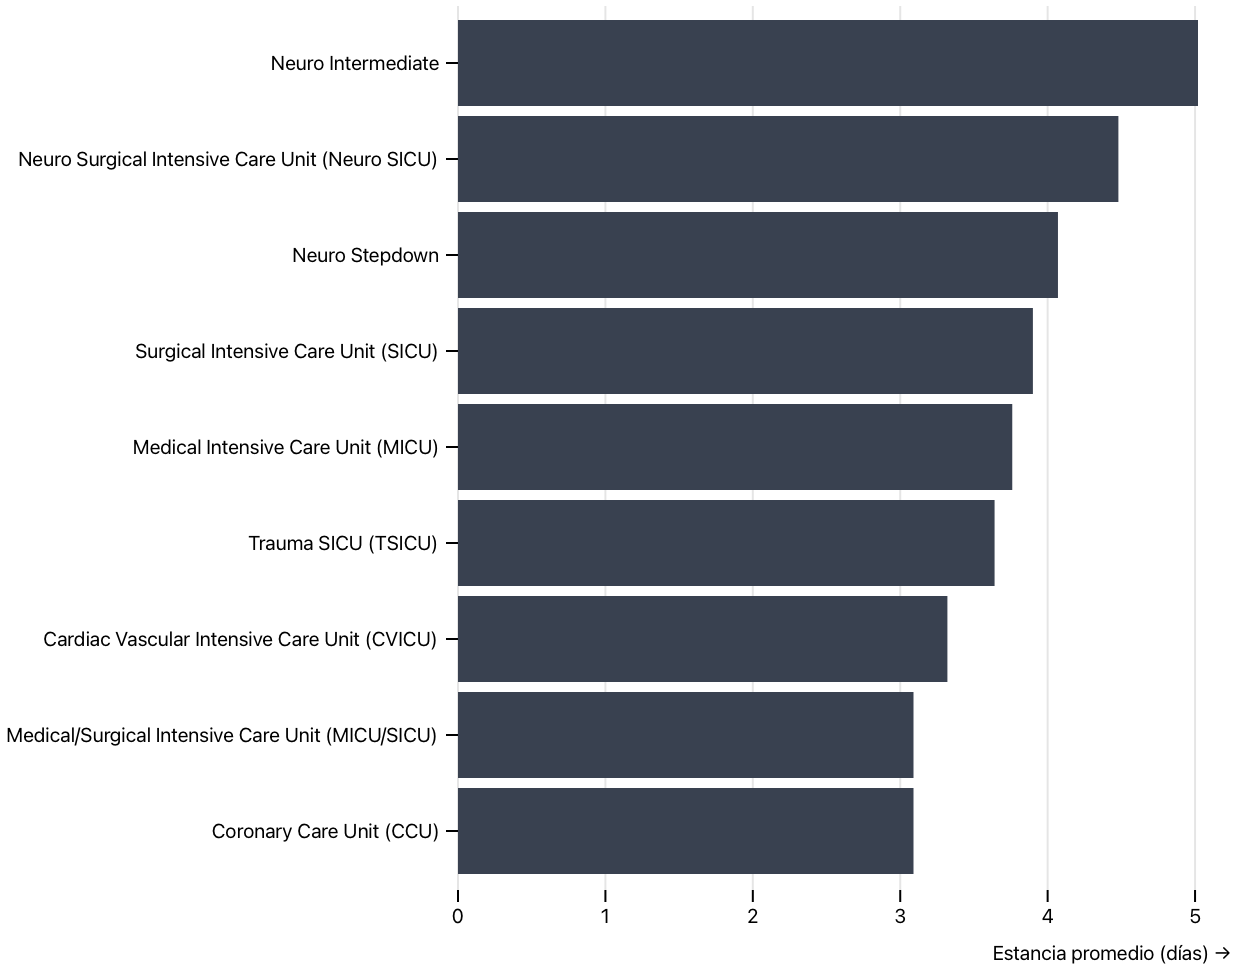
\includegraphics[width=0.65\textwidth]{imagenes/chart1.png}
  \caption{Estancia promedio por unidad UCI}
  \label{fig:chart1}
\end{figure}


\begin{figure}[H]
  \centering
  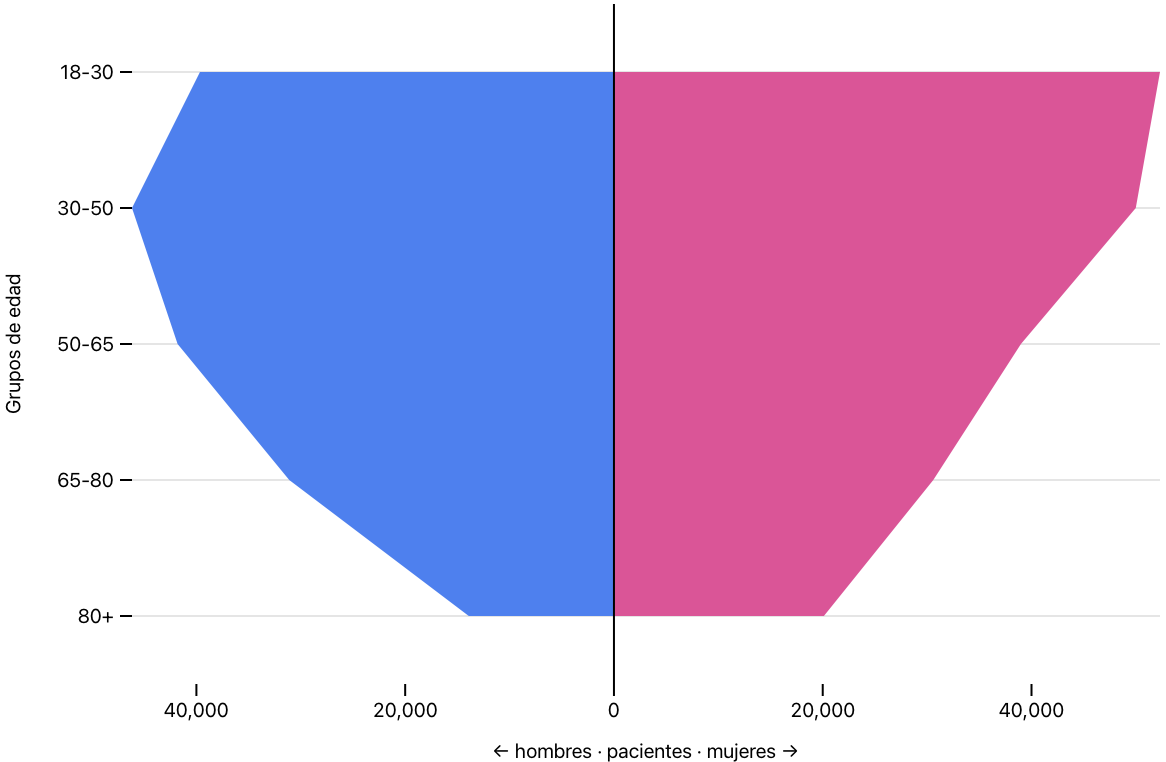
\includegraphics[width=0.65\textwidth]{imagenes/chart2.png}
  \caption{Distribución por edad y género (rangos de edad)}
  \label{fig:chart2}
\end{figure}

\begin{figure}[H]
  \centering
  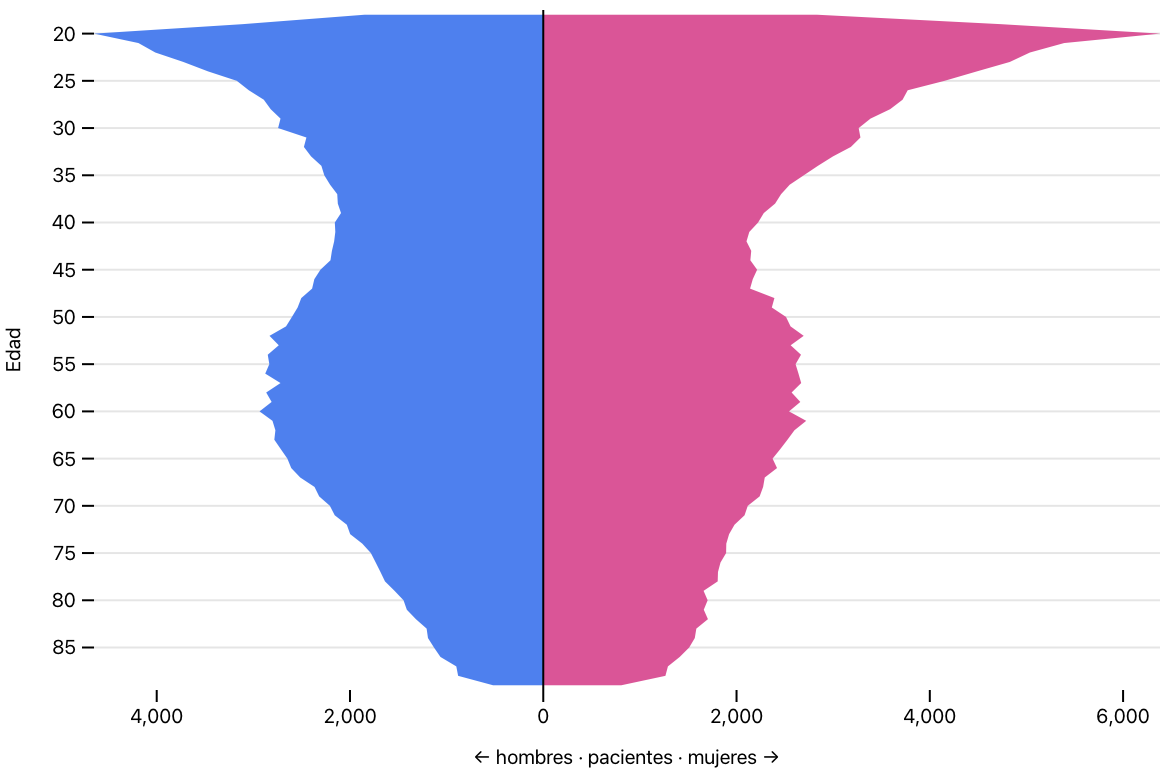
\includegraphics[width=0.65\textwidth]{imagenes/chart3.png}
  \caption{Distribución por edad y género}
  \label{fig:chart3}
\end{figure}






\begin{figure}[H]
  \centering
  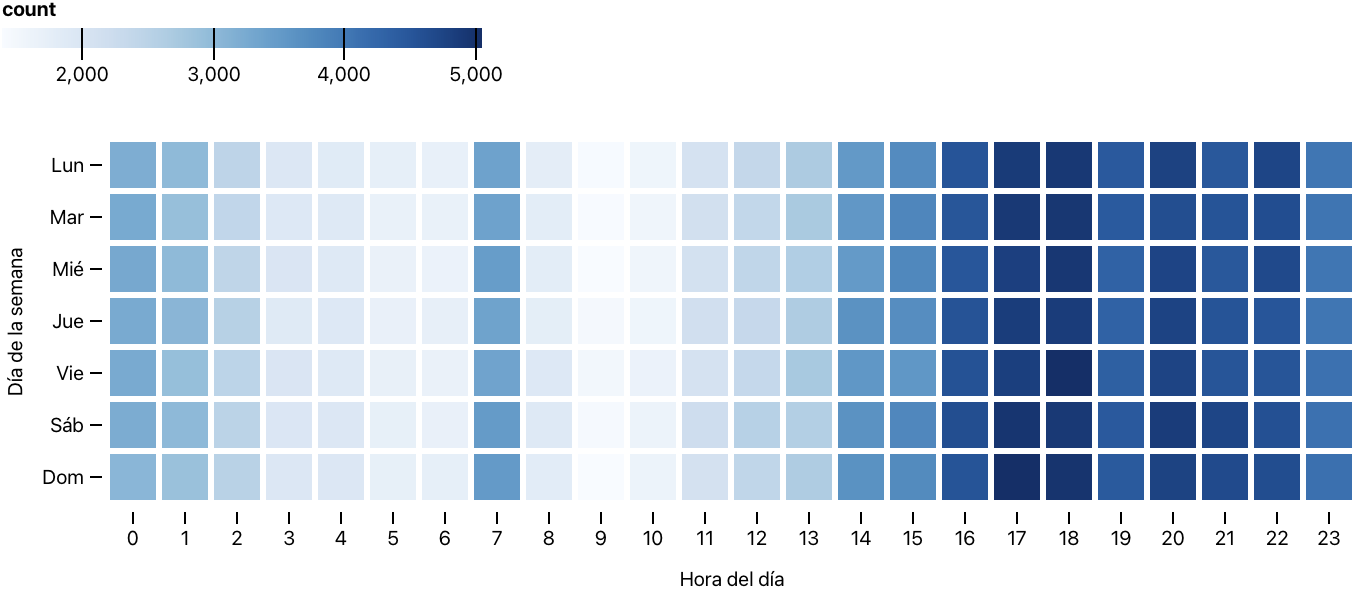
\includegraphics[width=0.8\textwidth]{imagenes/chart4.png}
  \caption{Heatmap de ingresos por hora y día de la semana}
  \label{fig:chart4}
\end{figure}


\begin{figure}[H]
  \centering
  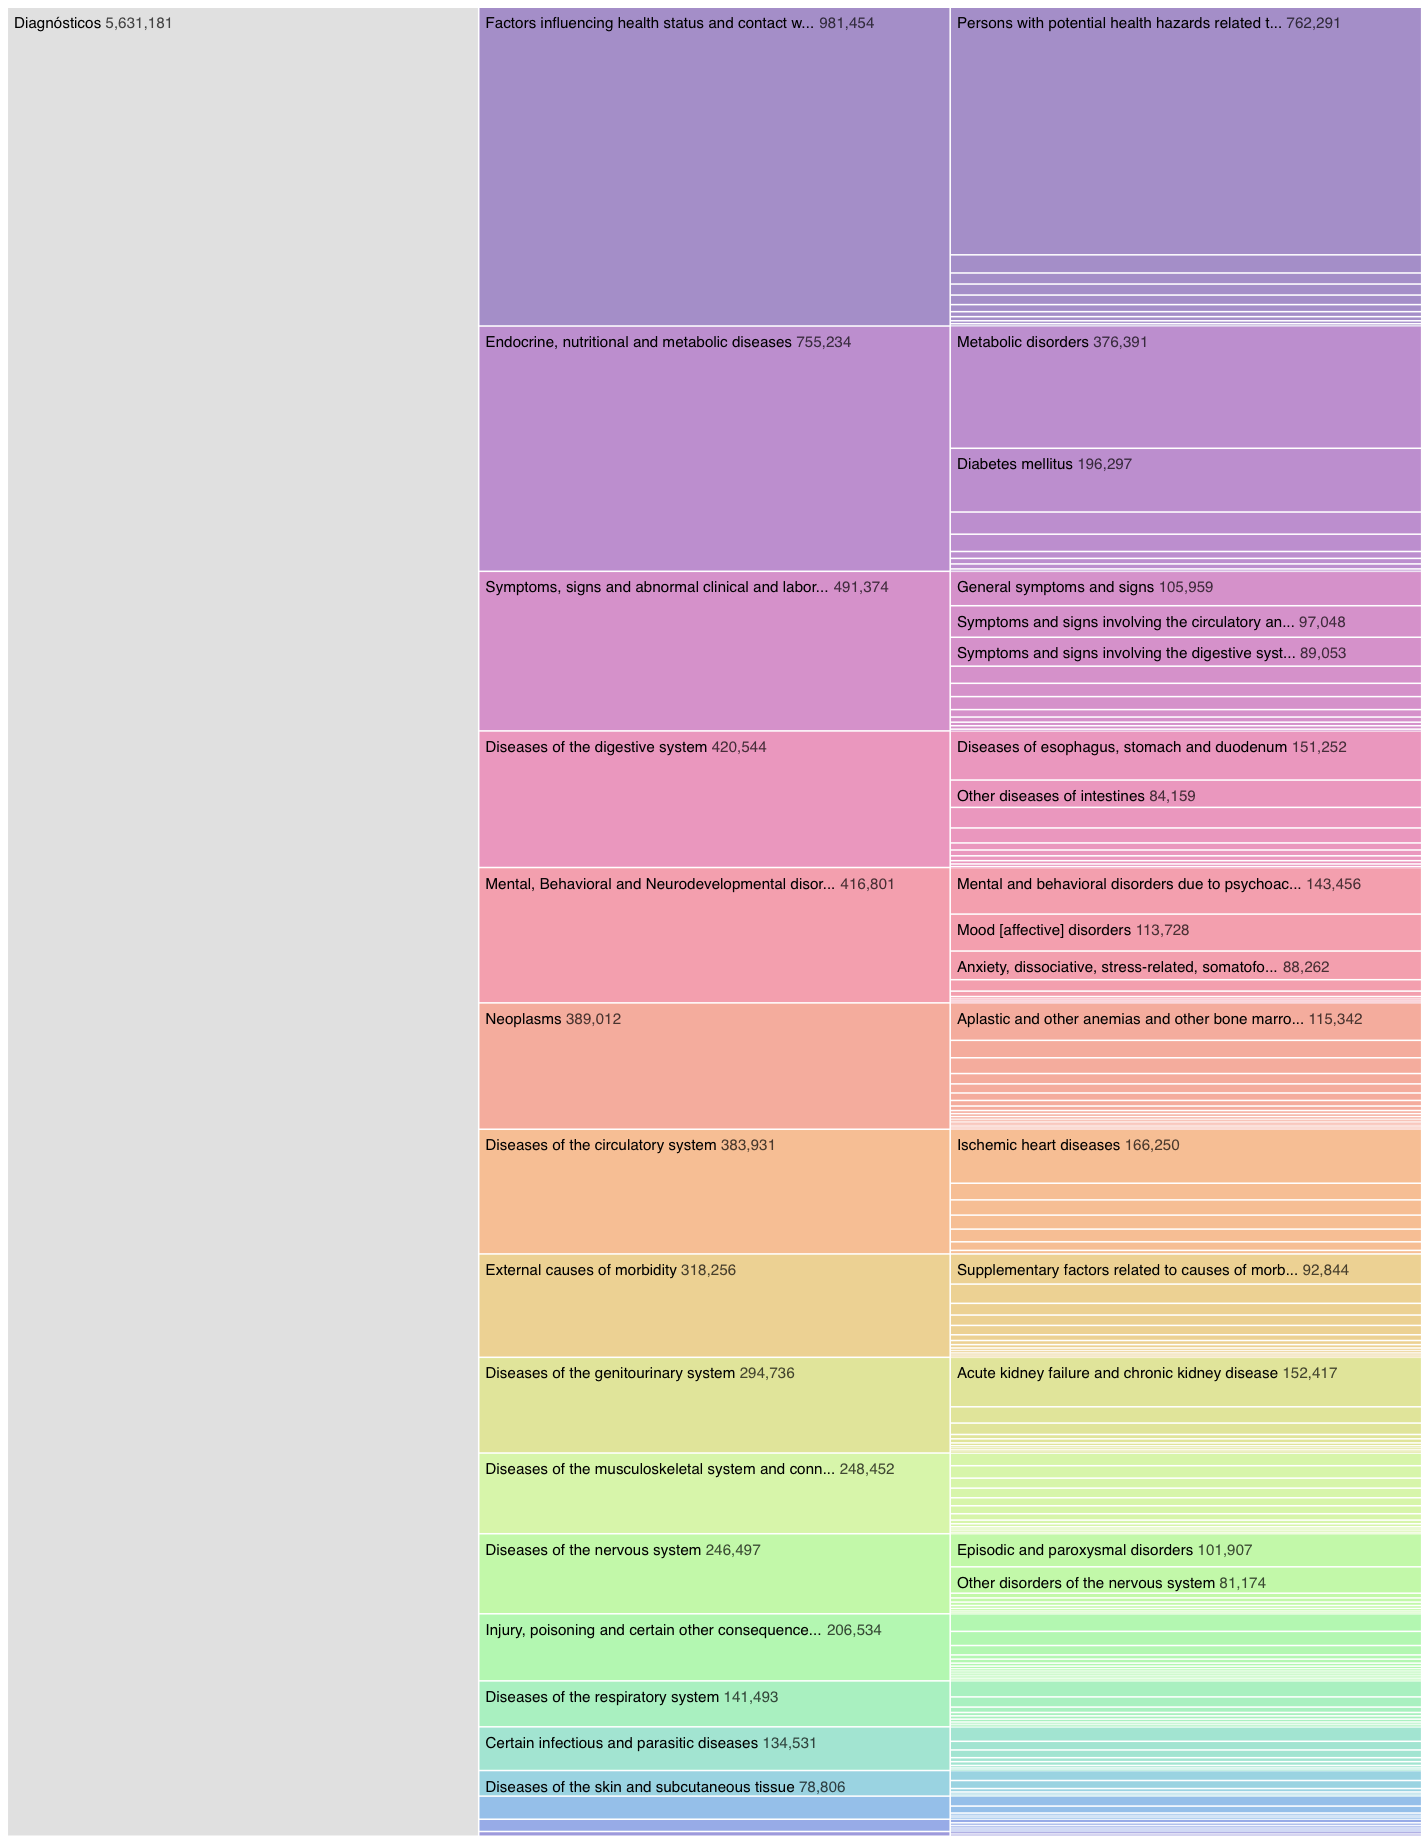
\includegraphics[width=0.88\textwidth]{imagenes/chart5.png}
  \caption{Zoomable icicle chart de diagnósticos por categoría}
  \label{fig:chart5}
\end{figure}

@todo: hablar de cada grafico la info que aporta?

@todo: explicar como seria el proceso de agregar un grafico nuevo?